\documentclass[12pt]{article} % 12pt 为字号大小 UTF8
\usepackage{amssymb,amsfonts,amsmath,amsthm}
%\usepackage{fontspec,xltxtra,xunicode}
%\usepackage{times}

%----------
% 定义中文环境
%----------

\usepackage{xeCJK}
\usepackage{color}
% \setCJKmainfont[BoldFont={SimHei},ItalicFont={KaiTi}]{SimSun}
% \setCJKsansfont{SimHei}
% \setCJKfamilyfont{zhsong}{SimSun}
% \setCJKfamilyfont{zhhei}{SimHei}

% \newcommand*{\songti}{\CJKfamily{zhsong}} % 宋体
% \newcommand*{\heiti}{\CJKfamily{zhhei}}   % 黑体


%----------
% 版面设置
%----------
%首段缩进
\usepackage{indentfirst}
\setlength{\parindent}{2.1em}

%行距
\renewcommand{\baselinestretch}{1.4} % 1.4倍行距

%页边距
\usepackage[a4paper]{geometry}
\geometry{verbose,
	tmargin=3cm,% 上边距
	bmargin=3cm,% 下边距
	lmargin=3cm,% 左边距
	rmargin=3cm % 右边距
}


%----------
% 其他宏包
\usepackage{listings}

%----------
%图形相关
\usepackage[x11names]{xcolor} % must before tikz, x11names defines RoyalBlue3
\usepackage{graphicx}
\usepackage{pstricks,pst-plot,pst-eps}
\usepackage{subfig}
\def\pgfsysdriver{pgfsys-dvipdfmx.def} % put before tikz
\usepackage{tikz}

%原文照排
\usepackage{verbatim}

%网址
\usepackage{url}
\usepackage[framed,numbered,autolinebreaks,useliterate]{mcode}

%----------
% 习题与解答环境
%----------
% %习题环境
% \theoremstyle{definition} 
% \newtheorem{exs}{习题}

% %解答环境
% \ifx\proof\undefined\
% \newenvironment{proof}[1][\protect\proofname]{\par
% \normalfont\topsep6\p@\@plus6\p@\relax
% \trivlist
% \itemindent\parindent
% \item[\hskip\labelsep
% \scshape
% #1]\ignorespaces
% }{%
% \endtrivlist\@endpefalse
% }
% \fi

% \renewcommand{\proofname}{\it{证明}}

%----------
% 我的自定义
%----------

\newcommand{\horrule}[1]{\rule[0.5ex]{\linewidth}{#1}} 	% Horizontal rule

\renewcommand{\refname}{参考文献}
\renewcommand{\abstractname}{\large \bf 摘\quad 要}
\renewcommand{\contentsname}{目录}
\renewcommand{\tablename}{表}
\renewcommand{\figurename}{图}

\setlength{\parskip}{0.4ex} % 段落间距

\usepackage{enumitem}
\setenumerate[1]{itemsep=0pt,partopsep=0pt,parsep=\parskip,topsep=5pt}
\setitemize[1]{itemsep=0.4ex,partopsep=0.4ex,parsep=\parskip,topsep=0.4ex}
\setdescription{itemsep=0pt,partopsep=0pt,parsep=\parskip,topsep=5pt}


%==========
% 正文部分
%==========

\begin{document}
	\title{
		%	{\normalfont\normalsize\textsc{
		%			Xiangtan University  \\[25pt]}}
		\horrule{0.5pt}\\
		\sffamily{数值最优化方法实验报告\\约束问题求解}
		\horrule{1.8pt}\\[20pt]
	}
	\author{米科润\quad 19信计二班\\201905755824}
	\date{\today} % 若不需要自动插入日期,则去掉前面的注释;{ } 中也可以自定义日期格式
	
	\begin{titlepage}
		\maketitle
		\vspace{30pt}
		\thispagestyle{empty}
	\end{titlepage}
	
	\tableofcontents
	\thispagestyle{empty}
	
	\newpage
	\setcounter{page}{1}
	
	\section{外点法}
	求解问题
	\[
	\begin{split}
	min &(x_1-1)^2+(x_1-x_2)^2+(x_2-x_3)^2\\
		s.t.& x_1(1+{x_2}^2)+{x_3}^4-4-3\sqrt{2}\\
		&-10\le x_i\le10,i=1,2,3\\
		&x_0=(2,2,2)^T\\
	\end{split}
	\]
	\indent 构建下述Matlab文件
	\begin{itemize}
		\item 目标函数obj.m
		\item 约束条件函数constrains.m
		\item 增广目标函数Al obj.m
		\item 罚函数compare.m
		\item 外点罚函数求解函数Al main.m
	\end{itemize}
	\begin{lstlisting}
	%%
	function f=obj(x)
	f=(x(1)-1)^2+(x(1)-x(2))^2+(x(2)-x(3))^4;
	end
	%%
	function [h,g]=constrains(x)
	h=x(1)*(1+x(2)^2)+x(3)^4-4-3*sqrt(2);
	g(1)=x(1)+10;
	g(2)=x(2)+10;
	g(3)=x(3)+10;
	g(4)=-x(1)+10;
	g(5)=-x(2)+10;
	g(6)=-x(3)+10;
	end
	%%
	function f=AL_obj(x)
	global pena N_equ N_inequ;
	h_equ=0;
	h_inequ=0;
	[h,g]=constrains(x);
	for i=1:N_equ
		h_equ=h_equ+h(i).^2;
	end
	for i=1:N_inequ
		h_inequ=h_inequ+(min(g(i),0)).^2;
	end
	f=obj(x)+pena*(h_equ+h_inequ);
	end
	%%
	function f=compare(x)
	global pena N_equ N_inequ;
	h_equ=0;
	h_inequ=0;
	[h,g]=constrains(x);
	for i=1:N_equ
		h_equ=h_equ+h(i).^2;
	end
	for i=1:N_inequ
		h_inequ=h_inequ+(min(g(i),0)).^2;
	end
	f=pena*(h_equ+h_inequ);
	end
	%%
	function [X,FVAL]=AL_main(x_al,N_equ,N_inequ)
	global pena N_equ N_inequ;
	pena=0.1;
	c_scale=2;
	e_al=1e-6;
	max_itera=100;
	out_itera=1;
	while out_itera<max_itera
		x_al0=x_al;
		[X,FVAL]=fminunc(@AL_obj,x_al0);
		x_al=X;
		if compare(x_al)<=e_al
			break;
		end
		pena=c_scale*pena;
		out_itera=out_itera+1;
	end
	X=x_al;
	FVAL=obj(X);
	end
	\end{lstlisting}
	\indent 构建main.m输入参数求解
	\begin{lstlisting}
		function main()
		clc;clear;
		x_al=[2,2,2];
		N_equ=1;
		N_inequ=6;
		[X,FVAL]=AL_main(x_al,N_equ,N_inequ);
		disp(X);disp(FVAL);
		end
	\end{lstlisting}
	\indent 结果如下
	\begin{figure}[ht]
		\centering
		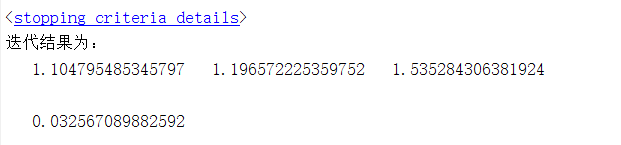
\includegraphics[width=0.8\textwidth]{waidian.png}
		\caption{外点罚函数法结果}
		\label{fig:fig1}
	\end{figure}
	\section{内点法}
	求解问题
	\[
	\begin{split}
	min &f(x)=-x_1x_2x_3\\
	s.t.& -{x_1}^2-2{x_2}^2-4{x_3}^2+48\ge0\\
	&x_0=(1,1,1)
	\end{split}
	\]
\indent 构建下述Matlab文件
\begin{itemize}
	\item 目标函数obj.m
	\item 约束条件函数constrains.m
	\item 增广目标函数Al obj.m
	\item 罚函数compare.m
	\item 外点罚函数求解函数Al main.m
\end{itemize}
\begin{lstlisting}
	%%
	function f=obj(x)
	f=-(x(1)*x(2)*x(3));;
	end
	%%
	function [h,g]=constrains(x)
	g=-x(1)^2-2*x(2)^2-4*x(3)^2+48;
	end
	%%
	function f=AL_obj(x)
	global pena N_inequ;
	h_inequ=0;
	g=constrains(x);
	for i=1:N_inequ
		h_inequ=h_inequ-log(g(i));
	end
	f=obj(x)+pena*(h_inequ);
	end
	%%
	function f=compare(x)
	global pena N_inequ;
	h_inequ=0;
	g=constrains(x);
	for i=1:N_inequ
		h_inequ=h_inequ-log(g(i));
	end
	f=pena*(h_inequ);
	end
	%%
	function [X,FVAL]=AL_main(x_al,N_equ,N_inequ)
	global pena N_equ N_inequ;
	pena=10;
	c_scale=0.5;
	e_al=1e-6;
	max_itera=100;
	out_itera=1;
	while out_itera<max_itera
		x_al0=x_al;
		[X,FVAL]=fminunc(@AL_obj,x_al0);
		x_al=X;
		if compare(x_al)<=e_al
			break;
		end
		pena=c_scale*pena;
		out_itera=out_itera+1;
	end
	X=x_al;
	FVAL=obj(X);
	end
\end{lstlisting}
\par{\textcolor{red}{问题:只有初始点非常靠近最优解时,所得结果近似正确}}\\
\indent 构建main.m输入参数求解
\begin{lstlisting}
	function main()
	clc,clear;
	x_al=[4,2*sqrt(2),2];
	N_inequ=1;
	[X,FVAL]=AL_main(x_al,N_inequ);
	disp(X);disp(FVAL);
	end
\end{lstlisting}
\indent 结果如下
\begin{figure}[ht]
	\centering
	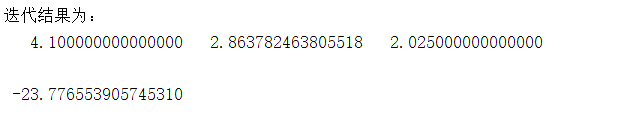
\includegraphics[width=0.8\textwidth]{neidian.png}
	\caption{内点罚函数法结果}
	\label{fig:fig1}
\end{figure}
		\section{乘子法}
	求解问题
	\[
	\begin{split}
		min &f(x)=-3{x_1}^2-{x_2}^2-2{x_3}^2\\
		s.t.& {x_1}^2+{x_2}^2+{x_3}^2=0\\
		&x_2\ge x_1\\
		&x_1\ge0\\
		&x_0=(0,0,0)^T
	\end{split}
	\]
	\indent 构建下述Matlab文件
	\begin{itemize}
		\item PHR算法函数multphr.m
		\item 增广拉格朗日函数mpsi.m
		\item 增广拉格朗日函数的梯度dmpsi.m
		\item 目标函数f1.m
		\item 等式约束函数h1.m
		\item 不等式约束函数g1.m
		\item 目标函数的梯度df1.m
		\item 等式约束的Jacob矩阵转置dh1.m
		\item 不等式约束的Jacob矩阵转置dg1.m
	\end{itemize}
	\begin{lstlisting}
		%%
		function [x,mu,lam,output]=multphr(fun,hf,gf,dfun,dhf,dgf,x0)
		theta=0.8;  eta=2.0;  
		k=0;  ink=0; 
		epsilon=1e-5; 
		x=x0;  he=feval(hf,x);  gi=feval(gf,x);
		n=length(x);  l=length(he);  m=length(gi)
		mu=0.1*ones(l,1);  lam=0.1*ones(m,1);
		betak=10;  betaold=10;  
		while(betak>epsilon & k<maxk)
		[ik,x,val]=bfgs('mpsi','dmpsi',x0,fun,hf,gf,dfun,dhf,dgf,...
		mu,lam,sigma);
		ink=ink+ik;
		he=feval(hf,x); gi=feval(gf,x);
		betak=sqrt(norm(he,2)^2+norm(min(gi,lam/sigma),2)^2);
		if betak>epsilon
			mu=mu-sigma*he;
			lam=max(0.0,lam-sigma*gi);
				if(k>=2 & betak>theta*betaold)
					sigma=eta*sigma;
				end
		end
		k=k+1;
		betaold=betak;
		x0=x;
		end
		f=feval(fun,x);
		output.fval=f;
		output.iter=k;
		output.inner_iter=ink;
		output.beta=betak;
		%%
		function psi=mpsi(x,fun,hf,gf,dfun,dhf,dgf,mu,lam,sigma)
		f=feval(fun,x);  he=feval(hf,x);  gi=feval(gf,x);
		l=length(he);  m=length(gi);
		psi=f;  s1=0.0;
		for(i=1:l)
			psi=psi-he(i)*mu(i);
			s1=s1+he(i)^2;
		end
		psi=psi+0.5*sigma*s1;
		s2=0.0;
		for(i=1:m)
			s3=max(0.0,lam(i)-sigma*gi(i));
			s2=s2+s3^2-lam(i)^2;
		end
		psi=psi+s2/(2.0*sigma);
		%%
		function dpsi=dmpsi(x,fun,hf,gf,dfun,dhf,dgf,mu,lam,sigma)
		dpsi=feval(dfun,x);
		he=feval(hf,x);  gi=feval(gf,x);
		dhe=feval(dhf,x);  dgi=feval(dgf,x);
		l=length(he);  m=length(gi);
		for(i=1:l)
			dpsi=dpsi+(sigma*he(i)-mu(i))*dhe(:,i);
		end
		for(i=1:m)
			dpsi=dpsi+(sigma*gi(i)-lam(i))*dgi(:,i);
		end
		%%
		function f=f1(x)
		f=-3*x(1)^2-x(2)^2-2*x(3)^2;
		end
		%%
		function he=h1(x)
		he=x(1)^2+x(2)^2+x(3)^2-3;
		end
		%%
		function gi=g1(x)
		gi=zeros(2,1);
		gi(1)=-x(1)+x(2);
		gi(2)=x(1);
		end
		%%
		function g=df1(x)
		g=[-6*x(1);-2*x(2);-4*x(3)];
		end
		%%
		function dhe=dh1(x)
		dhe=[2*x(1), 2*x(2), 2*x(3)]';
		end
		%%
		function dgi=dg1(x)
		dgi=[-1  1; 1 0; 0 0];
		end
	\end{lstlisting}
	\indent 命令窗口输入:
	\begin{lstlisting}
	x0=[0,0,0]';
	[x,mu,lam,output]=multphr('f1','h1','g1','df1','dh1','dg1',x0)
	\end{lstlisting}
	\indent 结果如下
	\begin{figure}[ht]
		\centering
		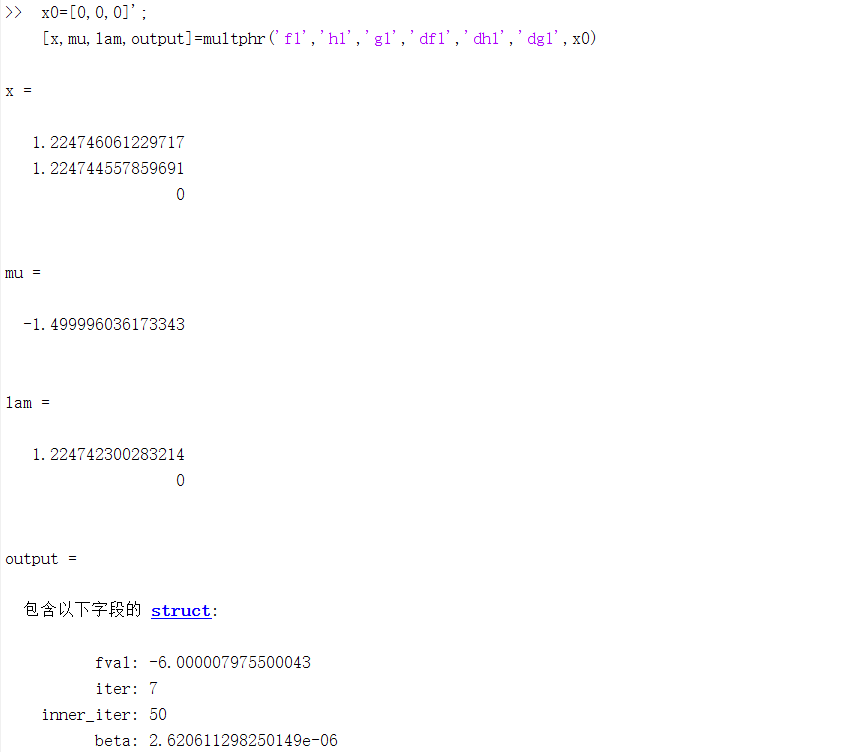
\includegraphics[width=0.8\textwidth]{phr.png}
		\caption{乘子法结果}
		\label{fig:fig1}
	\end{figure}
\end{document}